%!TEX root = ../main.tex

\section{Введение}

\begin{frame}{Физическое явление}
\begin{block}{Электрический пробой}
	Явление резкого возрастания тока в диэлектрике при приложении электрического напряжения выше критического.
\end{block}
\begin{itemize}
	\item Рассматриваем твердый диэлектрик
	\item Деградация диэлектрических свойств материала
	\item Процесс развивается в ограниченной зоне -- канале пробоя
	\item Сложная физическая природа
\end{itemize}
\end{frame}


\begin{frame}{Математическая модель}
\begin{block}{Модель типа диффузной границы}
	Вещество находится в разных фазах. Состояние вещества описывается гладкой функцией $\phi(\vx, t)$ -- фазовым полем.
\end{block}
\begin{itemize}
	\item $\phi = 1$ -- неповрежденная среда
	\item $\phi = 0$ -- полностью разрушенная среда
	\item Зона $\phi \in (0, 1)$ -- диффузная граница
	\item На разрушение среды тратится энергия
\end{itemize}
\begin{figure}
	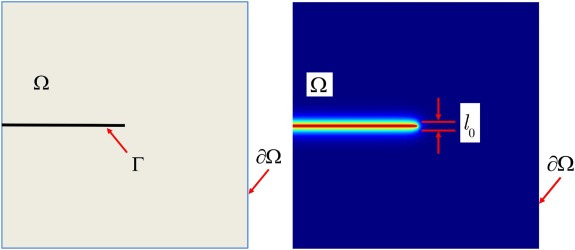
\includegraphics[width=0.5\textwidth]{figures/diffuse_edge.jpg}
\end{figure}
\end{frame}


\begin{frame}{Математическая модель}
\vspace{-0.3cm}
\begin{block}{Уравнения динамики системы}
	\begin{itemize}
		\item Уравнение электрического потенциала $\Phi$:
		\[
			\Div(\epsilon[\phi] \nabla \Phi) = 0
		\]
		\item Уравнение фазового поля $\phi$ (типа Аллена--Кана):
		\[
			\cfrac{1}{m} \partt{\phi} = \half \epsilon'(\phi) \gradsq{\Phi} + \cfrac{\Gamma}{l^2} f'(\phi) + \half \Gamma \Delta \phi
		\]
	\end{itemize}
\end{block}
\begin{itemize}
	\item Плотность свободной энергии
	\vspace{-0.2cm}
	\[
		\pi = -\half \epsilon[\phi] \gradsq{\Phi} + \Gamma \cfrac{1 - f(\phi)}{l^2} + \cfrac{\Gamma}{4} \gradsq{\phi}
	\]
\end{itemize}
\vspace{-0.6cm}
\begin{columns}
\column{0.33\textwidth}
	\vspace{0.35cm}
	\[
		f(\phi) = 4 \phi^3 - 3 \phi^4
	\]
\column{0.33\textwidth}
	\[
		\epsilon(\vx, t) = \cfrac{\epsilon_0(\vx)}{f(\phi(\vx, t)) + \delta}
	\]
\column{0.33\textwidth}
\end{columns}
\end{frame}

